%========== Heaps ==========%

\chapter{Heaps}
\label{ch:heaps}

\textbf{Pensum} 6 \cite{clrs} \\\\
\textbf{Assignments} 2-2 (counter example), 13-3 (tree relation) \\\\
\textbf{Algorithms} Heap-sort \\\\
\textbf{Keywords} Min- and maxheap, sorting, priority queues
\vspace{1in}

\noindent A heap is a nearly complete $n$-nary tree, we will concern ourselves
only with binary heaps - and as such, a binary heap is a nearly complete
binary tree. A heap implements a set $S$ of elements, in which each element
has an associated key. The actual structure of a heap is simply an array, and
so a heap is defined by the operations performed on the array, rather than the
data structure itself. The reason a heap is a tree-structure is a
visualization of the data, but not reflected by the data structure in any way.

Visualizing the array of a heap as a tree, we have that the root of the tree
corresponds to the first element of the array $i = 0$ (zero-indexed). The
parent of any node $n$ is given by $\lfloor n/2 \rfloor$. The children are
given by $2n$ and $2n + 1$, for left and right, respectively.

\newpage
\noindent Using the rules of traversal defined above, we can visualize the
array
\begin{figure}[H]
	\center
	\begin{tabular}{|c|c|c|c|c|c|c|c|c|c|}
		\hline 16 & 14 & 10 & 8 & 7 & 9 & 3 & 2 & 4 & 1 \\ \hline
	\end{tabular}
	\caption{Example of a (binary-)heap}
	\label{fig:heap-array}
\end{figure}
as a tree-structure, as shown in the following figure.
\begin{figure}[H]
	\center
	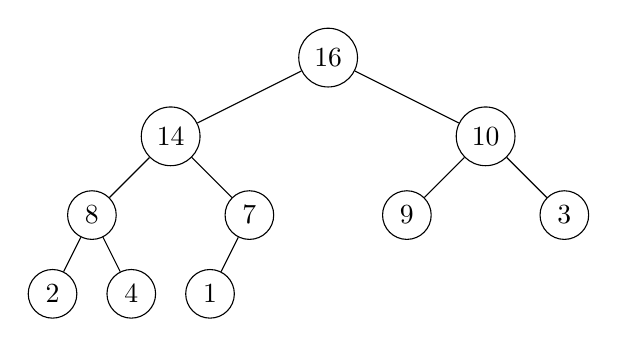
\begin{tikzpicture}
	[
	scale=1.0,
	align=center,
	every node/.style={circle, fill=white, draw=black}
	]
		% level 1
		\node (n1) at 	(3.5, -1) {16};
		
		% level 2
		\node (n2) at 	(1.5, -2) {14};
		\node (n3) at 	(5.5, -2) {10};
		
		% level 3
		\node (n4) at 	(0.5, -3) {8};
		\node (n5) at 	(2.5, -3) {7};
		\node (n6) at 	(4.5, -3) {9};
		\node (n7) at 	(6.5, -3) {3};
		
		% level 4
		\node (n8) at 	(0, -4) {2};
		\node (n9) at 	(1, -4) {4};
		\node (n10) at 	(2, -4) {1};
		% \node (n11) at 	(3, -4) {11};
		% \node (n12) at 	(4, -4) {12};
		% \node (n13) at 	(5, -4) {13};
		% \node (n14) at 	(6, -4) {14};
		% \node (n15) at 	(7, -4) {15};
		
		% drawing code
		\foreach \from/\to in {n1/n2,n1/n3} \draw (\from) -- (\to);
		\foreach \from/\to in {n2/n4,n2/n5,n3/n6,n3/n7} \draw (\from) -- (\to);
		\foreach \from/\to in {n4/n8,n4/n9,n5/n10} \draw (\from) -- (\to);
	\end{tikzpicture}
	\caption{Example of a (binary-)heap visualized as a tree}
	\label{fig:heap-tree}
\end{figure}

\section{Priority Queues}
\label{ch:heaps|sub:priorityqueues}
A priority queue is an abstract data structure, which sorts and maintains a
set of data in such a way, that the data is prioritized.A priority queue is not a destinct structure but a
class of data structures. Priority queues work well with stacks, heaps, self-organizing lists, etc. We will focus
mainly on heaps.
A heap is a priority queue and must adhere to the properties of either max or min-heap.
\begin{description}
	\item \textbf{Max-heap} The key of a node is greater than or equal to the
keys of its children.
	\item \textbf{Min-heap} The key of a node is less than or equal to the
keys of its children.
\end{description}
Max- and Min-Heaps are defined by their procedures, and we must show that their properties are maintained by those.

\clearpage

\begin{algorithm}[H]
	\caption{Max-heapify}
	\label{alg:max-heapify}
	
	\SetKwInOut{Input}{Input}
	\SetKwInOut{Output}{Output}
	
	\SetKwFunction{MaxHeapify}{MaxHeapify}
	\SetKwFunction{Left}{Left}
	\SetKwFunction{Right}{Right}
	
	\Input{An array $A$ and index $i$}
	\Output{In-place swapping max-heap property violations of $A$.}
	
	\BlankLine
	\MaxHeapify($A$, $i$) \\
	\Begin
	{
		$l = $ \Left($i$) \\
		$r = $ \Right($i$) \\
		$largest = i$ \\
		\If{$l \leq A.size $ \textnormal{and} $A[l] > A[i]$}
		{
			$largest = l$ \\
		}
		\If{$r \leq A.size $ \textnormal{and} $A[r] > A[largest]$}
		{
			$largest = l$ \\
		}
		\If{$largest \neq i$}
		{
			Swap $A[i]$ and $A[largest]$ \\
			\MaxHeapify($A$, $largest$)
		}
	}
\end{algorithm}
The procedure looks for a violation of the max-heap property, restoring it by
correcting that particular instance and check for further violations on the
corrected index.

Assuming the worst case, where the subproblem size is $2n/3$ we get the
recurrence $T(n) \leq T(2n/3) + \Theta(1)$, which by the master theorem (see
section \ref{eqn:master-theorem}) gives us $T(n) = O(\lg n)$, which
conveniently translates to the height of a tree - so for a given node $i$, we,
at most, correct a \textit{simple path} of the tree.
\\\\
\begin{algorithm}[H]
	\caption{Build max-heap}
	\label{alg:build-max-heap}
	
	\SetKwInOut{Input}{Input}
	\SetKwInOut{Output}{Output}
	\SetKwInOut{Invariant}{Invariant}
	
	\SetKwFunction{BuildMaxHeap}{BuildMaxHeap}
	\SetKwFunction{MaxHeapify}{MaxHeapify}
	
	\SetKw{DownTo}{ down to }
	
	\Input{An array $A$}
	\Output{In-place heapifying the array $A$.}
	\Invariant{At the start of each iteration, each node $i+1, i+2, \dots, n$
is the root of a max-heap.}
	
	\BlankLine
	\BuildMaxHeap($A$) \\
	\Begin
	{
		$A.size = A.length$ \\
		\For{$i = \lfloor A.length/2 \rfloor \DownTo 1$}
		{
			\MaxHeapify($A$, $i$)
		}
	}
\end{algorithm}
\noindent \textbf{Initialization} \\
Prior to the first iteration of the loop, $i = \lfloor n/2 \rfloor$. Each node
$\lfloor n/2 \rfloor + 1 \lfloor n/2 \rfloor + 2, \dots n$ is a leaf and is
thus the root of a trivial max-heap.
\\\\
\noindent \textbf{Maintenance} \\
Both children of node $i$ are higher than $i$, by the loop invariant, they are
then both roots of max-heaps. As we call \texttt{MaxHeapify} it correct any
violations of the max-heap property of these. Hence we are building levels of
the max-heap in a bottom-up fashion.
\\\\
\noindent \textbf{Termination} \\
At termination $i = 0$. By the loop invariant, each node $1, 2, \dots, n$ is
the root of a max-heap - in particular, node $1$ is.
\\\\
The initialization part of the algorithm on lines 1-3 take constant time
$\Theta(1)$, and since we call \texttt{MaxHeapify} $n/2$ times, we must have
that \texttt{BuildMaxHeap} is upper-bounded by $O(n \lg n)$.

We can tighten this bound by observing that \texttt{MaxHeapify} is dependent
on the height $h = \lfloor \lg n \rfloor$, and has at most $\lceil n/2^{h+1}
\rceil$ nodes.

We can then express the upper bound by
\begin{align}
	\sum_{h=0}^{\left\lfloor \lg n \right\rfloor}
	\lceil \frac {n}{2^{h+1}} \rceil O(h) =
	O \left( n \sum_{h=0}^{\lfloor \lg n \rfloor} \frac{h}{2^h} \right)
\end{align}
the last summation can be evaluated using the formula in appendix
\ref{appendix:equations|eqn:intdiff-series}, substituting $x = 1/2$, yielding
\begin{align}
	\sum_{h=0}^{\infty} \frac{h}{2^h} = \frac{1/2}{(1 - 1/2)^2} = 2
\end{align}
Thus, we can bound the running time of \texttt{BuildMaxHeap} as
\begin{align}
	O \left( n \sum_{h=0}^{\lfloor \lg n \rfloor} \frac{h}{2^h} \right) =
	O \left( n \sum_{h=0}^{\infty} \frac{h}{2^h} \right) = O(n)
\end{align}
Hence the running-time of building a max-heap from an unordered array can be
done in linear time.

\newpage

\section{Procedures}
\label{ch:heaps|sec:procedures}
These are the procedures that are supported by max- or min-heaps.

\subsection{Extraction}
\label{ch:heaps|sec:procedures|sub:extraction}
When we want to extract an element out of a heap, because of its practical use
we are typically interested only in the root node, which holds the maximum
key. Getting the root node is a trivial problem, we simply return the element
at index zero. \\
\begin{algorithm}[H]
	\caption{Extract max}
	\label{alg:heap-extract-max}
	
	\SetKwInOut{Input}{Input}
	\SetKwInOut{Output}{Output}
	
	\SetKw{Error}{error}
	
	\SetKwFunction{ExtractMax}{ExtractMax}
	\SetKwFunction{MaxHeapify}{MaxHeapify}
	
	\Input{A heap $A$.}
	\Output{Returns the maximum of a heap, removing it from the heap.}
	
	\BlankLine
	\ExtractMax($A$) \\
	\Begin
	{
		\If{$A.size < 1$}{ \Error "Heap underflow." }
		$max = A[1]$ \\
		$A[1] = A[A.size]$ \\
		$A.size = A.size - 1$ \\
		\MaxHeapify($A$, 1) \\
		\Return $max$
	}
\end{algorithm}
Lines 2-8 take constant time $\Theta(1)$, and as such the running-time of an
extraction operation is dictated by the call to \texttt{MaxHeapify}, which is
$O(\lg n)$.

\subsection{Increase key}
Increasing the priority of an entry is done using the following procedure. \\
\label{ch:heaps|sec:procedures|sub:increase-key}
\begin{algorithm}[H]
	\caption{Increase key}
	\label{alg:heap-increase-key}
	
	\SetKwInOut{Input}{Input}
	\SetKwInOut{Output}{Output}
	
	\SetKw{Error}{error}
	\SetKw{And}{ and }
	
	\SetKwFunction{IncreaseKey}{IncreaseKey}
	\SetKwFunction{Parent}{Parent}
	
	\Input{A heap $A$, an index $i$ and a key $k$.}
	\Output{Increases the key of index $i$ into the heap $A$ to the key $k$.}
	
	\BlankLine
	\IncreaseKey($A$, $i$, $k$) \\
	\Begin
	{
		\If{$k < A[i]$}{ \Error "New key is smaller than the current key" }
		$A[i] = k$ \\
		\While{$i < 1 $ \And $A[$ \Parent($i$) $] < A[i]$}
		{
			Swap $A[i]$ with $A[$ \Parent($i$) $]$ \\
			$i = $ \Parent($i$)
		}
	}
\end{algorithm}
Lines 2-6 take constant time $\Theta(1)$. Like \texttt{MaxHeapify} the
\texttt{while}-loop traces from the node, which in the worst case is a leaf,
to the root, which gives us a worst-case of $O(\lg n)$.

\subsection{Insertion}
Inserting a key into a heap is done using the following procedure. \\
\label{ch:heaps|sec:procedures|sub:insertion}
\begin{algorithm}[H]
	\caption{Heap insertion}
	\label{alg:heap-insert}
	
	\SetKwInOut{Input}{Input}
	\SetKwInOut{Output}{Output}
	
	\SetKwFunction{Insert}{Insert}
	\SetKwFunction{IncreaseKey}{IncreaseKey}
	
	\Input{A heap $A$ and a key $k$.}
	\Output{Inserts the key $k$ into the heap $A$.}
	
	\BlankLine
	\Insert($A$, $k$) \\
	\Begin
	{
		$A.size = A.size + 1$ \\
		$A[A.size] = -\infty$ \\
		\IncreaseKey($A$, $A.size$, $k$)
	}
\end{algorithm}
Lines 2-4 take constant time $\Theta(1)$, and thusly inherits its complexity
from the call to \texttt{IncreaseKey}, which is $O(\lg n)$.

\newpage
\section{Sorting}
Given that the procedure for extraction, as defined in section
\ref{ch:heaps|sec:procedures|sub:extraction}, one can easily imagine that
building a max- or min-heap and emptying the priority queue by repeatedly
calling the extraction procedure on it produces a sorted array.

\begin{algorithm}[H]
	\caption{Heapsort}
	\label{alg:heapsort}
	
	\SetKwInOut{Input}{Input}
	\SetKwInOut{Output}{Output}
	
	\SetKwFunction{HeapSort}{HeapSort}
	\SetKwFunction{BuildMaxHeap}{BuildMaxHeap}
	\SetKwFunction{MaxHeapify}{MaxHeapify}
	
	\SetKw{DownTo}{ down to }
	
	\Input{An unordered array $A$}
	\Output{In-place sorting of the array $A$.}
	
	\BlankLine
	\HeapSort($A$) \\
	\Begin
	{
		\BuildMaxHeap($A$) \\
		\For{$i = A.length \DownTo 2$}
		{
			Exchange $A[1]$ with $A[i]$ \\
			$A.size = A.size - 1$ \\
			\MaxHeapify($A$, 1)
		}
	}
\end{algorithm}

The initializing call to \texttt{BuildMaxHeap} takes $O(n)$ time, and each
$n-1$ calls to \texttt{MaxHeapify} takes $O(\lg n)$ time. Thus the running-
time of heap sort is $O(n \lg n)$.

